\graphicspath{{~/Cloud/thesis/latex/org/img/}}
\begin{tikzpicture}
  \tikzstyle{legend}=[draw, text width=4.2cm, align=center]

  \node[inner sep=0pt, anchor=south west] (assemblage) at (0,0)
  {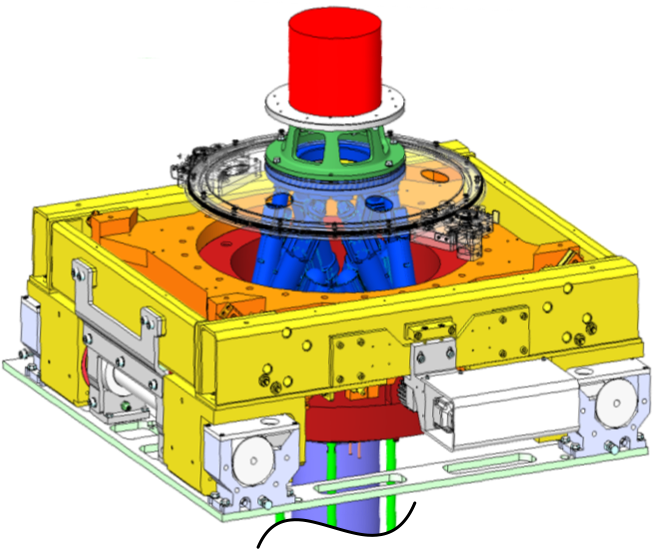
\includegraphics[width=0.42\textwidth]{/home/thomas/Cloud/thesis/papers/dehaeze18_sampl_stabil_for_tomog_exper/tikz/img/assemblage_img.png}};

  \coordinate[] (aheight) at (assemblage.north west);
  \coordinate[] (awidth)  at (assemblage.south east);

  \coordinate[] (xrightlabel) at (-0.2, 0);
  \coordinate[] (xleftlabel)  at ($(awidth)+(0.2, 0)$);

  % Translation Stage
  \coordinate[] (ty) at ($0.5*(aheight)+0.1*(awidth)$);
  \draw[<-] (ty) -- (ty-|xrightlabel) node[left, legend]{Translation Stage\\$\SI{-5}{m\metre} < T_y < \SI{5}{m\metre}$};

  % Sample Interface
  \coordinate[] (sampleint) at ($0.77*(aheight)+0.5*(awidth)$);
  \coordinate[] (sampleintmid) at ($(sampleint)+(-1, -0.5)$);
  \draw[<-] (sampleint) -- (sampleintmid) -- (sampleintmid-|xrightlabel) node[left, legend]{Sample Interface};

  % Sample
  \coordinate[] (sample) at ($0.9*(aheight)+0.5*(awidth)$);
  \draw[<-] (sample) -- (sample-|xrightlabel) node[left, legend]{Sample Environment\\$\SI{1}{\kg} < M < \SI{50}{\kg}$};

  % Tilt Stage
  \coordinate[] (tilt) at ($0.55*(aheight)+0.78*(awidth)$);
  \coordinate[] (tiltmid) at ($(tilt)+(1, 0.5)$);
  \draw[<-] (tilt) -- (tiltmid) -- (tiltmid-|xleftlabel) node[right, legend]{Tilt Stage\\$\ang{-3} < \theta_y < \ang{3}$};

  % Spindle
  \coordinate[] (spindle) at ($0.53*(aheight)+0.33*(awidth)$);
  \coordinate[] (spindlemid) at ($(spindle)+(-1, -1.5)$);
  \draw[<-] (spindle) -- (spindlemid) -- (spindlemid-|xrightlabel) node[left, legend]{Spindle\\$\SI{1}{rpm} < \dot{\theta_z} < \SI{60}{rpm}$};

  % Center of gravity compensation
  \coordinate[] (axisc) at ($0.65*(aheight)+0.65*(awidth)$);
  \coordinate[] (axiscmid) at ($(axisc)+(1, 1.5)$);
  \draw[<-] (axisc) -- (axiscmid) -- (axiscmid-|xleftlabel) node[right, legend]{Center of gravity\\compensation system};

  % Micro Hexapod
  \coordinate[] (hexapod) at ($0.52*(aheight)+0.6*(awidth)$);
  \coordinate[] (hexapodmid) at ($(hexapod)+(1, -1.0)$);
  \draw[<-] (hexapod) -- (hexapodmid) -- (hexapodmid-|xleftlabel) node[right, legend]{Long Stroke Hexapod\\$\SI{-10}{m\metre} < T_{x y z} < \SI{10}{m\metre}$\\$\ang{-3} < \theta_{x y z} < \ang{3}$};

  % Frame
  \coordinate[] (frame) at ($0.14*(aheight)+0.65*(awidth)$);
  \draw[<-] (frame) -- (frame-|xleftlabel) node[right, legend]{Frame fixed\\on the granite};

  % X-Ray
  \draw[color=red, ->-=0.7] ($0.92*(aheight)+0.8*(awidth)$) -- node[above, color=black]{X-ray} ++(190:1.8);

  % Size of the setup
  \draw[dashed, <->, color=black!70, line width=0.5pt] ($0.03*(aheight)+0.35*(awidth)$) -- node[below, color=black, pos=0.6]{$\approx\SI{1}{m}$} ($0.14*(aheight)+0.98*(awidth)$);
  \draw[dashed, <->, color=black!70, line width=0.5pt] ($0.032*(aheight)+0.32*(awidth)$) -- node[left, color=black, pos=0.4]{$\approx\SI{1}{m}$} ($0.305*(aheight)+0.0*(awidth)$);

  % Axis
  \begin{scope}[shift={(0.0, 0.7)}]
    \draw[->] (0, 0) -- ++(195:0.8) node[above] {$x$};
    \draw[->] (0, 0) -- ++(90:0.9) node[right] {$z$};
    \draw[->] (0, 0) -- ++(-40:0.7) node[above] {$y$};
  \end{scope}

\end{tikzpicture}
